\section{Persistent Homology}

%-------------------------------------------------------------------------------

\subsection{Filtration}

\begin{definition}
    Let $K$ be a simplicial complex. A filtration on $K$ is a sequence of simplicial complexes:
    $$
    \emptyset = K_0 \subseteq K_1 \subseteq \ldots \subseteq K_n = K.
    $$
\end{definition}

\begin{example}
    Let $K$ be the Delaunay triangulation of a finite set $S \subseteq \R^2$. For each simplex $\sigma \in K$ there is a real number $\alpha_\sigma$ such that $\sigma$ belongs to $A(\alpha)$ if and only if $\alpha_\sigma \leq \alpha$. We can order the n simplices in $K$, first by dimension, then within each dimension group using the order induced by $\alpha_{\sigma_1} \leq \alpha_{\sigma_2} \leq \ldots \alpha_{\sigma_n}$. This gives a filtration on $K$:
    $$
    \emptyset = K_0 \subseteq K_1 \subseteq \ldots \subseteq K_n = K.
    $$
    This filtration is called flat because any two contiguous complexes differ by a single simplex. Since every alpha complex is a subcomplex of the Delaunay triangulation, every alpha complex belongs to this triangulation. Moreover $\alpha \leq \alpha'$ implies $A(\alpha) \subseteq A(\alpha')$
\end{example}

%-------------------------------------------------------------------------------

\subsection{Birth and Death}

Let $K_0 \subseteq K_1 \subseteq \ldots \subseteq K_n$ be a filtration. For $i \leq j$ there is an inclusion $f^{i, j}: K_i \hookrightarrow K_j$. This map induces an inclusion homomorphism $f_p^{i, j}: Z_p(K_i) \hookrightarrow Z_p(K_j)$, which in turn induces the homomorphism 
$$
\phi_p^{i, j}: H_p(K_i) \rightarrow H_p(K_J).
$$
The image of $\phi_p^{i, j}$ is called a persistent homology group. It contains all the p-dimensional homology classes from $K_i$ that are still present in $K_j$. 

We say a class $\gamma \in H_p(K_i)$ is born at $K_i$ if it's not in the image of $\phi_p^{i-1, i}$, and a class born in $K_i$ dies entering $K_{j+1}$ if $\phi_p^{i, j}(\gamma)$ isn't in the image of $\phi_p^{i-1, j}$ but $\phi_p^{i, j+1}(\gamma)$ is in the image of $\phi_p^{i-1, j+1}$. The intuition behind the second part of this definition is that we characterise the death of a class as it being subsumed by a class which existed prior to its birth. The first part of this definition is to ensure this subsumption happens exactly at $K_{j+1}$ and not before.

The index of persistence of $\gamma$ is $j + 1 - i$. Often we have a function which governs the construction of the filtration. Let $b$ be the value of the function at a classes birth and $d$ the value at its death. We call $(b, d)$ a birth death pair, and difference $d - b$ the persistence of the class. In an alpha complex filtration, this would be the extension of $\sigma \mapsto \alpha_{\sigma}$ to the filtration (which is possible because it is flat).

%-------------------------------------------------------------------------------

\subsection{Barcodes}

A barcode plot is a convenient way to represent the birth and death of classes throughout a filtration. In its unrestricted form, each horizonal bar represents a generator of the homology group, its length and position represent when, and for how long, it was alive. Bars which extend to the right hand edge of the diagram are those which persisted to the end of the filtration. 

The number of bars tends to get large when the data has more complicated topology. We tend to simplify the diagram by placing restrictions on the minimum length of bars we'd like to include, or the total number of bars.

The following plot shows a simplified barcode plot for 1000 points sampled from a torus. Importantly, we can see that a single bar in the zeroth homology class extends to infinity - which represents the single connected component of a torus, and two bars in the first homology class that extend to infinity represent the generators of $Z \times Z = H_1(T^2)$.

\begin{center}
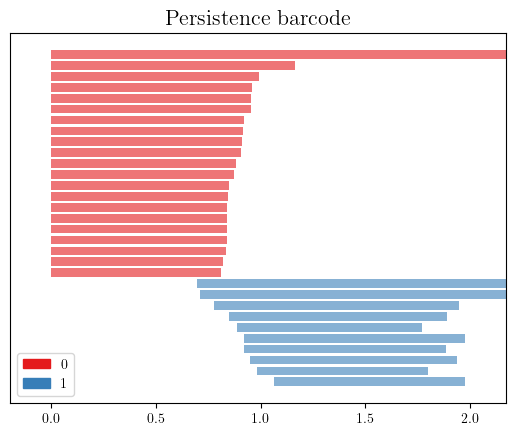
\includegraphics[scale=0.8]{figures/torus_barcode.png}
\end{center}

%-------------------------------------------------------------------------------

\subsection{Peristence Diagrams}

As mentioned, barcode diagrams can become extremely complicated for data with more complex topology. For these cases, a representation as points in the plane is convenient. In a peristence diagram we plot birth time against death time with each point representing a generator from a homology class. Points are colour coded by the homology group they belong to.

The following plot shows a persistence diagram for 1000 points sampled froma  torus. The points close to the line $y = x$ represent generators which which died shortly after being born. Those far away from this line represent generators which persisted for longer. We can again see some of the important topological features of the torus encoded in the diagram.

\begin{center}
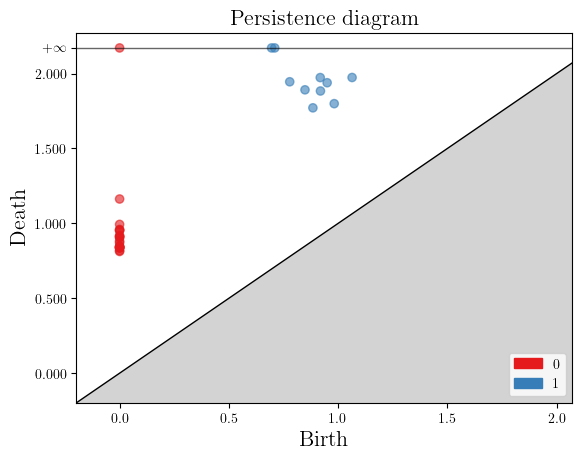
\includegraphics[scale=0.8]{figures/torus_persistence_diagram.png}
\end{center}

We now define a metric on the space of persistence diagrams.

\begin{definition}
    Let $\mathcal{D}$ and $\mathcal{D}'$ be persistence diagrams. Define the Bottleneck distance between them as 
    $$
    W_{\infty}(\mathcal{D}, \mathcal{D}') = \inf_{\mu: \mathcal{D} \rightarrow \mathcal{D}'} \max_{x \in \mathcal{D}} \norm{x - \mu(x)}_{\infty},
    $$ 
    where $\mu$ is a bijection. 
\end{definition}

\begin{definition}
    Similarly, we define the p-th Wasserstein distance as 
    $$
    W_{p}(\mathcal{D}, \mathcal{D}') = \inf_{\mu: \mathcal{D} \rightarrow \mathcal{D}'} \sum_{x \in X} \norm{x - \mu(x)}_{\infty}^q.
    $$ 
\end{definition}

Also, we can define the following norms of a persistence diagram:

\begin{definition}
    $$
    \norm{\mathcal{D}}_{\infty} = \max_{x, y \in \mathcal{D}} \norm{x - y},
    $$
\end{definition}

\begin{definition}
    $$
    \norm{\mathcal{D}}_p = \sqrt[p]{\sum_{x, y \in \mathcal{D}} \norm{x - y}^p}.
    $$
\end{definition}

%-------------------------------------------------------------------------------

\subsection{Peristence Landscapes}

Fix a filtration, and consider the birth death pairs $\{(b_i, d_i)\}_{i=1}^n$ for a fixed homology dimension $p$. For each birth and death pair $(b, d)$, define the piecewise linear function $f_{(b, d)}: \R \rightarrow \infty$ by
$$
f_{(b, d)} = \begin{cases}
                0 & x \not\in (b, d) \\
                x - b & x \in (b, \frac{b + d}{2}) \\
                d - x & x \in (\frac{b + d}{2}, d).
             \end{cases}
$$
So $f_{(b, d)}$ is a steeple function, with the steeple on $(b, d)$, and the height of the steeple proportional to $d - b$

Define the pth persistence landscape of the data as $L: N \times \R \rightarrow [0, \infty)$ by setting $L(k, x)$ as the kth largest of the values $\{f_{(b_i, d_i)}(x)\}_{i=1}^n$, and $0$ if $k$ exceeds $n$.

%-------------------------------------------------------------------------------